\section{Exercise 1}

Consider the C program below, which is affected by a typical buffer overflow vulnerability.
\begin{verbnobox}[\verbarg]
#include <stdio.h>
#include <stdlib.h>
#include <string.h>

void vuln() {
    char buf[32];

    scanf("%s", buf);
    if (strncmp(buf, "Knight_King!", 12) != 0) {
        abort();
    }
}

int main(int argc, char** argv) {
    vuln();
}
\end{verbnobox}
\begin{enumerate}
    \item Assume that the program runs on the usual IA-32 architecture (32-bits), with the usual \texttt{cdecl} calling convention. 
        Also assume that the program is compiled without any mitigation against exploitation (ASLR is off, stack is executable, and stack canary is not present).
        Draw the stack layout when the program is executing the instruction at line seven, showing:
        \begin{itemize}
            \item Direction of growth and high-low addresses.
            \item The name of each allocated variable.
            \item The boundaries of frame of the function frames (\texttt{main} and \texttt{vuln}).
        \end{itemize}
        Show also the content of the caller frame.
    \item Write an exploit for the buffer overflow vulnerability in the above program. 
        Your exploit should execute the following simple shell code, composed only by four instructions: \texttt{0x12 0x34 0x56 0x78}.
        Write clearly all the steps and assumptions you need for the exploitation, and show the stack layout right after the execution of the \texttt{scanf()} during the program exploitation.
\end{enumerate}

\subsection*{Solution}
\begin{enumerate}
    \item To represent the stack layout described, we need to allocate space for the \texttt{buf} array, the saved EBP, and the saved EIP:
        \begin{figure}[H]
            \centering
            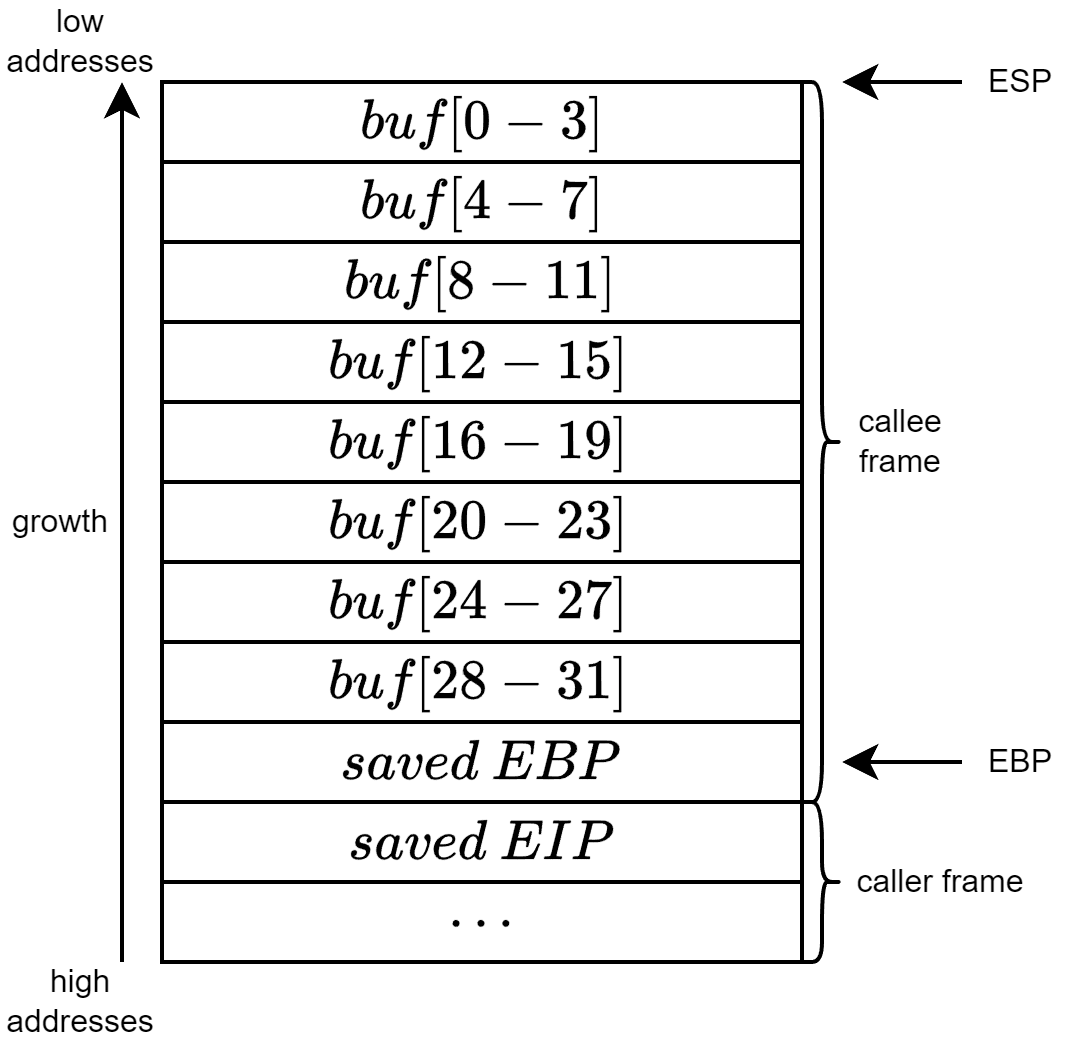
\includegraphics[width=0.5\linewidth]{images/stack.png}
        \end{figure}
    \item The stack in this case is: 
        \begin{figure}[H]
            \centering
            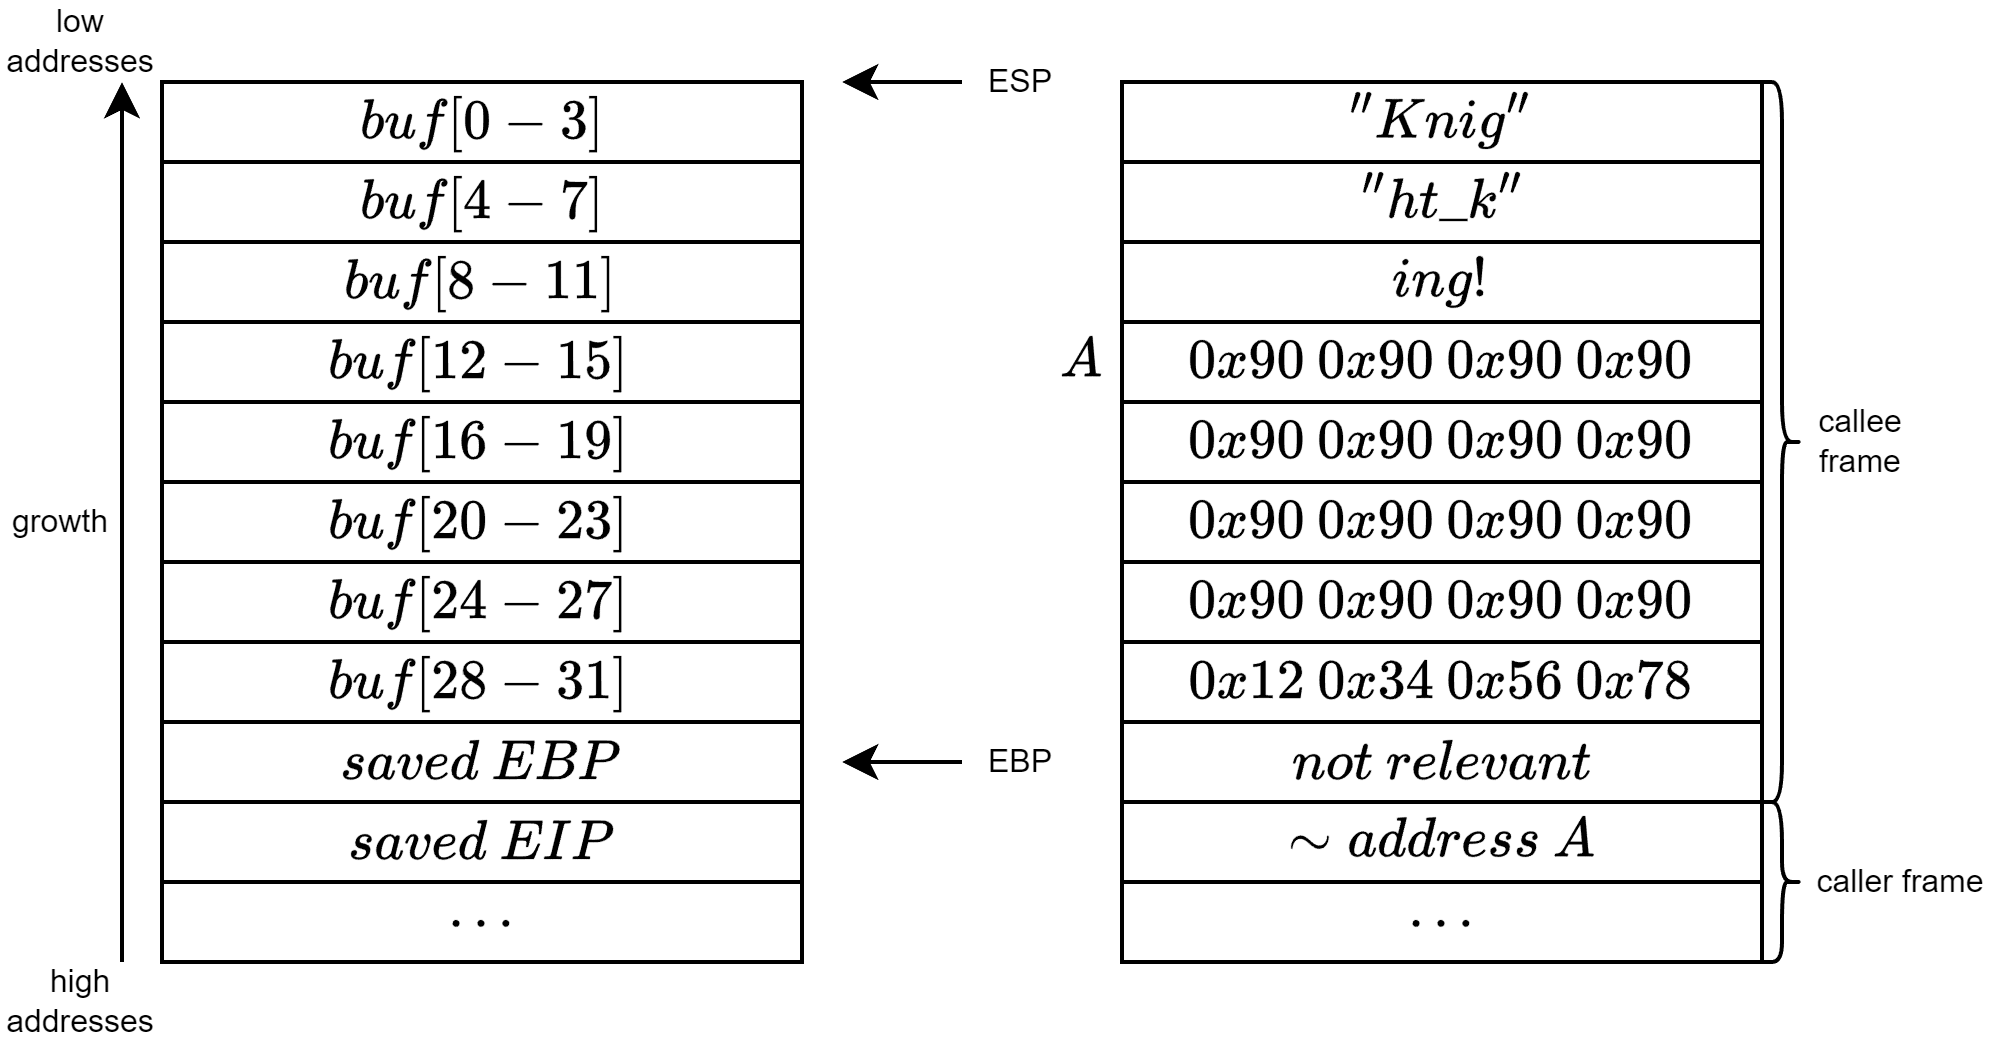
\includegraphics[width=0.75\linewidth]{images/stack1.png}
        \end{figure}
        In this layout:
        \begin{itemize}
            \item The first 16 bytes (four cells) are filled with no-operation instructions to avoid any unintended actions.
            The next 8 bytes (two cells) are reserved for the \texttt{buf} array.
            The following 4 bytes (one cell) are allocated for the saved EBP.
            The last 4 bytes (one cell) contain the address of the shell code.
        \end{itemize}
        The first twelve characters of \texttt{buf} are ensured to be different from "Knight\_King!" to avoid invoking \texttt{abort()}.
\end{enumerate}